\documentclass[12pt]{article}
\usepackage{placeins}		% Used to keep images in place(via \FloatBarriers), and let text go infront
\usepackage{graphicx} 		% Used to for importing images
\usepackage{indentfirst}	% Indents 1st paragraph (by default its off)
\usepackage{longtable} 		% Tables than can span over multiple pages

\setlength{\parindent}{20pt}

\begin{document}

\begin{titlepage}

% Defines a new command to draw horizontal lines
\newcommand{\Line}{\rule{\linewidth}{0.5mm}} 

% Center everything on the page
\center
 
% textsc - capitalizes every letter
\textsc{\LARGE University of Gothenburg}
% Define gap after text line
\\[3.5cm] 

% Course code and name
\textsc{\Large DIT168}\\[0.3cm]
\textsc{\large Project: Industrial IT and Embedded Systems}\\[0.5cm]

% Use the defined command to draw lines
\Line \\[0.4cm]
{\huge \bfseries Risk Management Document}\\[0.4cm]
\Line \\[0.5cm]
 
% Large italic text
\Large \textit{Authors:}
\\Erik Laurin
\\Isabelle Törnqvist
\\Joacim Eberlen
\\Justinas Stirbys \\[4cm]

% Original date for the document
{\large Group 01} \\[0.3cm]
{\large April 16th, 2018}

% Fills the remaining page with whitespace
\vfill

\end{titlepage}

% Creating table of contents
\tableofcontents
\pagebreak

% DOC start

% Add DOC history of changes table
\section{Revision History}
The evolution of the Risk Management Document for project dashFTABs is detailed under this section. Emphasis is put on changes incorporated, via Description column, the date and the author. In situation where all members have contributed to a change the author will be listed as Group 01.
% Define 4 aligned columns; l = left, c = center, r = right, the | = means vertical line    % \hline -> Draw horizontal line
% p{xcm} -> specifies how much space the column should take up, 
% 0.x\linewidth is used to make it p{} command more dynamic
\begin{longtable}{ | p{0.15\linewidth} | p{0.15\linewidth} | p{0.5\linewidth} | p{0.2\linewidth} | }\hline 
    
    \textbf{Date} & \textbf{Version} & \textbf{Description} & \textbf{Author} \\ \hline
    15th April, 2018 & 0.1 & Added Risk list & Erik Laurin,  Justinas Stirbys\\ \hline
   	18th May, 2018 & 0.2 & Added Heat Map & Justinas Stirbys\\ \hline

\end{longtable}
\pagebreak

\iffalse
% Identified risks section
\section{Identified risks}
Several risks that may arise throughout development were identified. \par
\fi

% Risk list section
\section{Risk List}
Numerous risks that may interfere with the development's continuation are identified and evaluated, see table 1 below. For each risk, its impact, probability and magnitude are estimated and presented in the table. See the key below for details on these paradigms. 

% Key for table below in bullet points form
\begin{itemize}
\item I - (impact). Impact is a numerical value, usually between 1 and 5, that represents the impact to the project if the risk comes true. 5 is a HIGH IMPACT and 1 is LOW IMPACT.
\item P - (probability). Probability is the percentage chance that a risk will occur.
\item M - (magnitude). Magnitude is the result of the multiplication of Probability and Impact, providing a joint metric suitable for sorting.
\end{itemize}
\par

% Risk list table
\begin{longtable}{| p{0.06\linewidth} | p{0.20\linewidth} | p{0.25\linewidth} | p{0.04\linewidth} | p{0.05\linewidth} | p{0.05\linewidth} | p{0.35\linewidth}|}
\caption{Risk Table}
\label{Risk Table}
\endfirsthead
\endhead
\hline

\textbf{Risk ID} & 
\textbf{Headline} & 
\textbf{Description} & 
\textbf{I} & 
\textbf{P} & 
\textbf{M} & 
\textbf{Mitigation Strategy}
\\ \hline

   	R1 & 
Developers lacking key skills & 
The team’s lack of knowledge and skills pertaining to Docker and C++ could cause an array of problems leading to lower product quality and customer value. & 
3 & 
75\% & 
2.25 &
Obtain as much knowledge as possible about these tools before the development phase. Continue using these tools throughout the project and as a group deal with potential issues acting as blocking states. Acquire assistance from teaching assistants; 'TAs', in case the development team gets stuck. \\ \hline
 
    	R2 & 
Lack of commitment & 
Meaning that possibly some team members may experience distractions taking away their focus from the project and leading them to accomplish less than expected. & 
3 & 
50\% & 
1.5 &
Use the resources provided to us, for example lectures, TAs and online guides. The team will attempt to focus on communication and improved planning. If the risks cannot be solved within the team, the teaching assistance will be asked for guidance. \\ \hline
   	
	R3 & 
Failed to meet deadlines &
Developers are not able to implement assigned features, test and verify them prior to established deadlines. &
4 & 
50\% & 
2 &
Always have a 'soft deadline' an appropriate time before the actual deadline. In case this soft deadline is not met, additional emergency meetings prior to the hard deadline will take place in order to make sure that the actual deadline is met and necessary resources are assigned. \\ \hline

	R4 & 
Lack of time &
Developers are unable to allocate enough time for the project, due to time constraints set upon by other courses, work, exam and/or life in general. &
4 & 
75\% & 
3 &
Use pair programming to improve developer efficiency and project velocity. Assign multiple developers for key tasks, in case one becomes unavailable. Have an open dialogue within the team to know one another's status. \\ \hline

	R5 & 
Developers clash &
The risk is an extreme case of Disagreement Amongst Stakeholders. The risk is surrounding developers fighting and animosity towards each other getting in the way of progress.&
4 & 
10\% & 
0.4 &
Attempt to have a reasonable discussion and work talk things out. If needed involve teaching assistants. \\ \hline

	R6 & 
Hardware faults &
The provided hardware; the car, starts to malfunction due to hardware faults. This has happened to other development teams. &
4 & 
40\% & 
0.4 &
Confront TAs immediately with the problem to make sure it is taken cared of as soon as possible. If the car gets unavailable over a longer time, prioritize development of features that do not, somehow, require direct access to the car. Last resort, borrow another group's car. \\ \hline

	R7 & 
Unable to find another group to test autonomous driving with (based on V2V protocol) &
No other group can be found to allow us to try our implementation of the autonomous driving (follow/leading) &
4 & 
50\% & 
2 &
Have a continuous dialogue with other groups to coordinate and facilitate testing between the groups. Yet, if not possible, mock another car with a computer. \\ \hline

	R8 & 
Poor accuracy when following leader car &
The car performs poorly when following another car &
3 & 
90\% & 
2.7 &
Check for obvious mistakes in the code. Identify where the problem lies through troubleshooting and deducing and cooperate with other groups too improve accuracy \\ \hline

	R9 & 
V2V protocol has critical shortcomings &
The mutual protocol does not suffice to allow following &
5 & 
10\% & 
0.5 &
Talk to development group's V2V responsible who will present the potential issues to the rest of the V2V responsible. Discuss within the development team strategies to mend the shortcoming. \\ \hline

	R10 & 
Message overflow &
The car struggles to handle the amount of messages &
4 & 
20\% & 
0.8 &
Eliminate unnecessary redundant message broadcasting. Utilize more than one OD4 session. Fine-tune the broadcast frequency of different services. \\ \hline
\end{longtable}
\pagebreak

%%%%%%%%%%%%%%%%%%%%%%%%%%%%%%%%
%%% New Section
%%%%%%%%%%%%%%%%%%%%%%%%%%%%%%%%
\section{Heat Map}
To visualize the possible project risks a heat map was made, for the purpose of improved visualization. The individual risks are represented via blue dots, the size varying based on their magnitude. The most severe risks are located at the top-right corner, whereas the least at the bottom-left corner. \par
Risks R3 \& R7 have the same Impact and Likilihood, therefore they have identical position on the graph. To compensate for this, the label for R3 has been positioned above the risk dot. Moreover, most of the risk are located to concentrated i
% Adding image
\FloatBarrier % -> Wrap image with this, to make sure text does not go in front of image if theres room
\begin{figure}[ht!]
\centering
% Make image as wide as the line
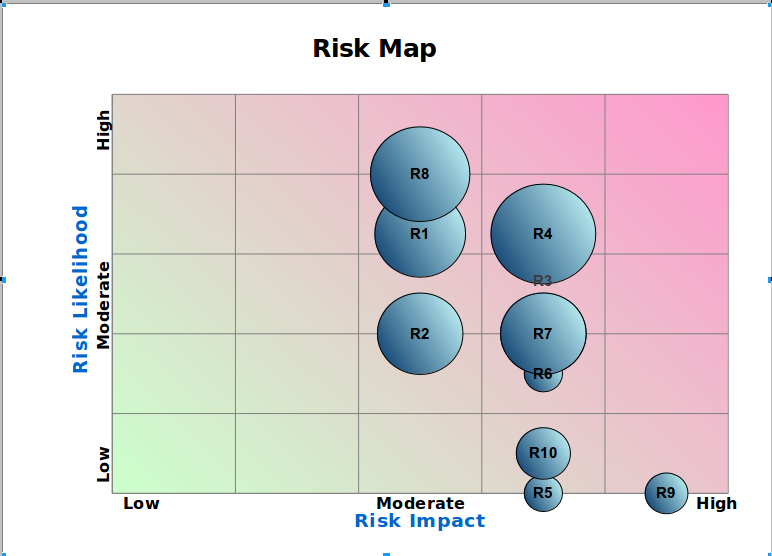
\includegraphics[width=\linewidth]{RiskMap.png}
\caption{Risk Heat Map}
\label{fig:heatmap}
\end{figure}
\FloatBarrier % -> Wrap image with this, to make sure text does not go infront of image if theres room

%%%%%%%%%%%%%%%%%%%%%%%%%%%%%%%%
%%% New Section
%%%%%%%%%%%%%%%%%%%%%%%%%%%%%%%%
\section{Risk Evaluation}
The purpose of this section is to go through the risks in Table \ref{Risk Table}, and to evaluate their mitigation stategies. \par 
Risk R1 was encountered during the project, but it is not believed to have as a significant impact as initially believed. The mitigation stategy for the risk seemed to work fine as the project group manage to attain knowledge about Docker and CMake before work with the cars begain. Additionally, the development team would utilize the offered Q\&A session to get access to the TAs for help and guidance. \par
R6 apperared as the miniature vehicle unable to turn right. The mitigation stategies for this issue did not work as the "right turn" issue persisted until the conclusion of the project. Moreover, it was not possible to borrow a new car. However, the mitigation stategies did work on other hardware issues that were less severe.  \par
The last major risk encountered is identified as R8. Although, the mitigation stategy outlined was not of the most concrete it did provide value. During W17 the development team worked closely with another group. The solution to having following be as close as possible was to impose a controlled environment. Meaning the development teams used the same network to test and present, the distance between starting car were measured and the alligned of the cars at the start were controller. Moreover, the development team encorporated a number of command line parameters to attempt to make the code as dynamic as possible for the purpose of fine tuning the V2V following. \par
Risks R2 and R5, relating to team communication did not occur, as there were no major conflicts during the project. Furthermore, R7 did not occur as the development team found 2 teams to test the V2V-Protocol and V2V following.  \par
R3 and R4 were not present in the project, since all hard deadlines were met. Moreover, the brunt of the project started on Study Period 2, meaning the development team was not hindered by other courses or exams as initially thought. \par
The identified V2V-Protocol risks, R9 and R10 were not present either. Although, there were minor protocol issues that were addressed and fixed, due to the project team being allowed to tailor the protocol to an extent.
\end{document}
